\subsubsection{UC\theuccount-GP - Producer GitLab invia messaggio al Gestore Personale}
	\begin{figure}[H]
		\centering
		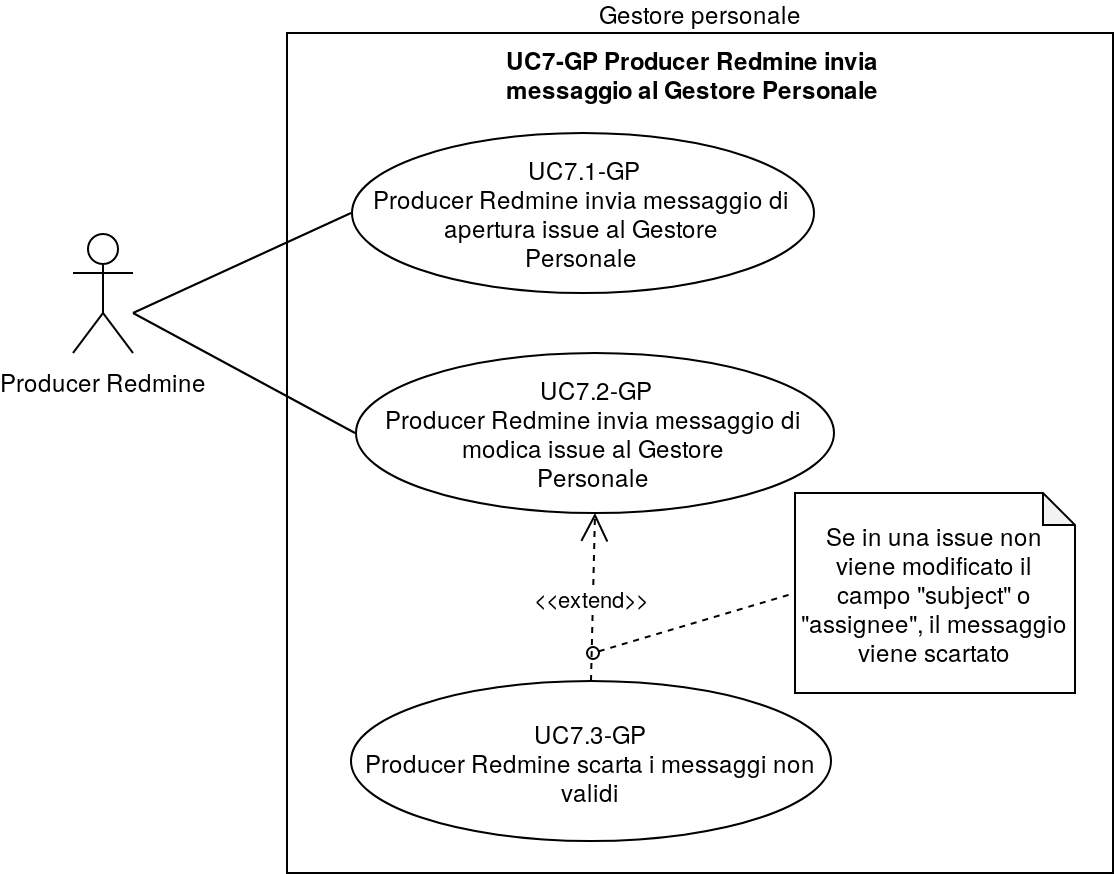
\includegraphics[width=0.7\textwidth]{img/casi_d'uso/UC7.png}\\
		\caption{UC\theuccount-GP - Producer GitLab invia messaggio al Gestore Personale}
	\end{figure}
	\begin{itemize}
		\item \textbf{Codice}: UC\theuccount-GP.
		\item \textbf{Titolo}: Producer GitLab invia messaggio al Gestore Personale.
		\item \textbf{Attori primari}: Producer GitLab.
		\item \textbf{Descrizione}: il Producer GitLab, dopo aver ricevuto una segnalazione da GitLab, elabora un messaggio da inviare al Gestore Personale. \\ Il messaggio elaborato conterrà i campi:
		\begin{itemize}
			\item App
			\item Object\_kind
			\item Title
			\item Project\_id
			\item Project\_name
			\item Author
			\item Assignees
			\item Action
			\item Description
			\item Labels
			\item Changes
		\end{itemize}
		\item \textbf{Precondizione}: il Producer GitLab ha ricevuto una segnalazione da GitLab.
		\item \textbf{Postcondizione}: il Producer GitLab ha inviato al Gestore Personale il messaggio  \newline elaborato.
		\item \textbf{Scenario principale}: 
		\begin{enumerate}
			\item Il Producer GitLab riceve una segnalazione da GitLab
			\item Il Producer GitLab prepara il messaggio in modo che venga inserito correttamente nel Gestore Personale
			\item Il Poducer GitLab invia il messaggio al Gestore Personale
            \item Il Gestore Perosonale riceve il messaggio dal Producer GitLab 
		\end{enumerate}
		
	\end{itemize}

	\stepcounter{subuccount}

	\subsubsection{UC\theuccount.\thesubuccount-GP - Producer GitLab invia messaggio di push al Gestore Personale}
		
		\begin{itemize}
			\item \textbf{Codice}: UC\theuccount.\thesubuccount-GP.
			\item \textbf{Titolo}: Producer GitLab invia uno o più messaggi di commit al Gestore Personale.
			\item \textbf{Attori primari}: Producer GitLab.
			\item \textbf{Descrizione}: il Producer GitLab, dopo aver ricevuto una segnalazione di push da  \newline GitLab, suddivide la segnalazione per i commit in più messaggi che verranno catalogati sotto il Topic "commits".
			\item \textbf{Precondizione}: il Producer GitLab ha ricevuto una segnalazione da GitLab.
			\item \textbf{Postcondizione}: il Producer GitLab ha inviato uno o più messaggi di commit.
			\item \textbf{Scenario principale}: 
			\begin{enumerate}
				\item Il Producer GitLab riceve la segnalazione di un push da GitLab
				\item Il Producer GitLab prepara i messaggi in modo che vengano inseriti correttamente nel Gestore Personale
				\item Il Producer GitLab invia i messaggi di
				commit al Gestore Personale
                \item Il Gestore Personale riceve i messaggi di commit
			\end{enumerate}
			\item \textbf{Estensioni}: 
			\begin{enumerate}
				\item Se ci sono dei messaggi non validi, questi vengono scartati [UC\theuccount.6-GP].
			\end{enumerate}
		\end{itemize}

	\stepcounter{subuccount}

	\subsubsection{UC\theuccount.\thesubuccount-GP - Producer GitLab invia messaggio di una nuova issue al Gestore Personale}
	
	\begin{itemize}
		\item \textbf{Codice}: UC\theuccount.\thesubuccount-GP.
		\item \textbf{Titolo}: Producer GitLab invia messaggio di una nuova issue al Gestore Personale.
		\item \textbf{Attori primari}: Producer GitLab.
		\item \textbf{Descrizione}: il Producer GitLab, dopo aver ricevuto una segnalazione di una nuova issue da GitLab, elabora il messaggio da inoltrare al Gestore Personale.
		\item \textbf{Precondizione}: il Producer GitLab ha ricevuto una segnalazione da GitLab.
		\item \textbf{Postcondizione}: il Producer GitLab ha inviato al Gestore Personale il messaggio
		elaborato di nuova issue.
		\item \textbf{Scenario principale}: 
		\begin{enumerate}
			\item Il Producer GitLab riceve la segnalazione di una nuova issue da GitLab
			\item Il Producer GitLab prepara il messaggio di una nuova issue in modo che venga inserito correttamente
			nel Gestore Personale
			\item Il Producer GitLab invia il messaggio di una nuova issue al Gestore Personale
		\end{enumerate}
		\item \textbf{Estensioni}: 
		\begin{enumerate}
			\item Se ci sono dei messaggi non validi, questi vengono scartati [UC\theuccount.6-GP].
		\end{enumerate}
	\end{itemize}
		
	\stepcounter{subuccount}
	
	\subsubsection{UC\theuccount.\thesubuccount-GP - Producer GitLab invia messaggio di modifica di una issue al Gestore Personale}
		\begin{itemize}
			\item \textbf{Codice}: UC\theuccount.\thesubuccount-GP.
			\item \textbf{Titolo}: Producer GitLab invia messaggio di modifica di una issue al Gestore Personale.
			\item \textbf{Attori primari}: Producer GitLab.
			\item \textbf{Descrizione}: il Producer GitLab, dopo aver ricevuto una segnalazione di issue da GitLab, controlla se la issue è appena stata creata o si tratta della modifica di una issue preesistente. Il messaggio, una volta elaborato, conterrà i campi:
			\begin{itemize}
				\item Project
                \item Author
				\item Topic
				\item Subject e opzionalmente:
				\begin{itemize}
					\item Description
					\item Due Date
					\item Milestone
					\item Assignee
				\end{itemize}
			\end{itemize}
			\item \textbf{Precondizione}: il Producer GitLab ha ricevuto una segnalazione da GitLab.
			\item \textbf{Postcondizione}: il Producer GitLab ha inviato al Gestore Personale il messaggio
			elaborato di modifica issue.
			\item \textbf{Scenario principale}: 
			\begin{enumerate}
				\item Il Producer GitLab riceve la segnalazione di issue da GitLab
				\item Il Producer GitLab prepara il messaggio di modifica issue in modo che venga inserito correttamente nel Gestore Personale
				\item Il Producer GitLab invia il messaggio di issue al Gestore Personale
                \item Il Gestore Personale riceve il messaggio di issue dal Producer GitLab
			\end{enumerate}
			\item \textbf{Estensioni}: 
			\begin{enumerate}
				\item Se ci sono dei messaggi non validi, questi vengono scartati [UC\theuccount.6-GP].
			\end{enumerate}
		\end{itemize}
		
		\stepcounter{subuccount}
		
		\subsubsection{UC\theuccount.\thesubuccount-GP - Producer GitLab invia messaggio di commento di una issue al Gestore Personale}
		\begin{itemize}
			\item \textbf{Codice}: UC\theuccount.\thesubuccount-GP.
			\item \textbf{Titolo}: Producer GitLab invia messaggio di commento di una issue al Gestore Personale.
			\item \textbf{Attori primari}: Producer GitLab.
			\item \textbf{Descrizione}: il Producer GitLab, dopo aver ricevuto una segnalazione di commento di una issue da GitLab, elabora il messaggio da inoltrare al Gestore Personale.
			\item \textbf{Precondizione}: il Producer GitLab ha ricevuto una segnalazione da GitLab.
			\item \textbf{Postcondizione}: il Producer GitLab ha inviato al Gestore Personale il messaggio
			elaborato di commento issue.
			\item \textbf{Scenario principale}: 
			\begin{enumerate}
				\item Il Producer GitLab riceve la segnalazione di commento issue da GitLab
				\item Il Producer GitLab prepara il messaggio di commento issue in modo che venga inserito correttamente nel Gestore Personale
				\item Il Producer GitLab invia il messaggio di commento issue al Gestore Personale
			\end{enumerate}
			\item \textbf{Estensioni}: 
			\begin{enumerate}
				\item Se ci sono dei messaggi non validi, questi vengono scartati [UC\theuccount.6-GP].
			\end{enumerate}
		\end{itemize}
		
		\stepcounter{subuccount}
		
		\subsubsection{UC\theuccount.\thesubuccount-GP - Producer GitLab invia messaggio di commento di un commit al Gestore Personale}
		\begin{itemize}
			\item \textbf{Codice}: UC\theuccount.\thesubuccount-GP.
			\item \textbf{Titolo}: Producer GitLab invia messaggio di commento di un commit al Gestore Personale.
			\item \textbf{Attori primari}: Producer GitLab.
			\item \textbf{Descrizione}: il Producer GitLab, dopo aver ricevuto una segnalazione di commento di un commit da GitLab, elabora il messaggio da inoltrare al Gestore Personale.
			\item \textbf{Precondizione}: il Producer GitLab ha ricevuto una segnalazione da GitLab.
			\item \textbf{Postcondizione}: il Producer GitLab ha inviato al Gestore Personale il messaggio
			elaborato di commento commit.
			\item \textbf{Scenario principale}: 
			\begin{enumerate}
				\item Il Producer GitLab riceve la segnalazione di commento commit da GitLab
				\item Il Producer GitLab prepara il messaggio di commento commit in modo che venga inserito correttamente nel Gestore Personale
				\item Il Producer GitLab invia il messaggio di commento commit al Gestore Personale
			\end{enumerate}
			\item \textbf{Estensioni}: 
			\begin{enumerate}
				\item Se ci sono dei messaggi non validi, questi vengono scartati [UC\theuccount.6-GP].
			\end{enumerate}
		\end{itemize}
		
		\stepcounter{subuccount}
		
		\subsubsection{UC\theuccount.\thesubuccount-GP - Producer GitLab scarta i messaggi non validi}
			
			\begin{itemize}
				\item \textbf{Codice}: UC\theuccount.\thesubuccount-GP.
				\item \textbf{Titolo}: Producer GitLab scarta i messaggi non validi.
				\item \textbf{Attori primari}: Producer GitLab.
				\item \textbf{Descrizione}: il Producer GitLab, dopo aver ricevuto un messaggio da GitLab, controlla
                che il messaggio contenga una segnalazione che \progetto\ sappia analizzare. In caso negativo, il messaggio viene scartato.
                \item \textbf{Precondizione}: il Producer GitLab ha ricevuto un messaggio da GitLab.
                \item \textbf{Postcondizione}: il Producer GitLab ha scartato il messaggio.
                \item \textbf{Scenario principale}: 
                \begin{enumerate}
                    \item Il Producer GitLab riceve un messaggio
                    \item Il Producer GitLab vede che il messaggio contiene una segnalazione che \progetto\ non sa analizzare
                    \item Il Producer GitLab scarta il messaggio non valido.
                \end{enumerate}
            \end{itemize}